\section{Referencia de la Clase Descuento\-Presupuesto}
\label{classDescuentoPresupuesto}\index{DescuentoPresupuesto@{DescuentoPresupuesto}}
Administra el descuento en un presupuesto.  


{\tt \#include $<$descpresupuesto.h$>$}

Diagrama de colaboraci\'{o}n para Descuento\-Presupuesto:\begin{figure}[H]
\begin{center}
\leavevmode
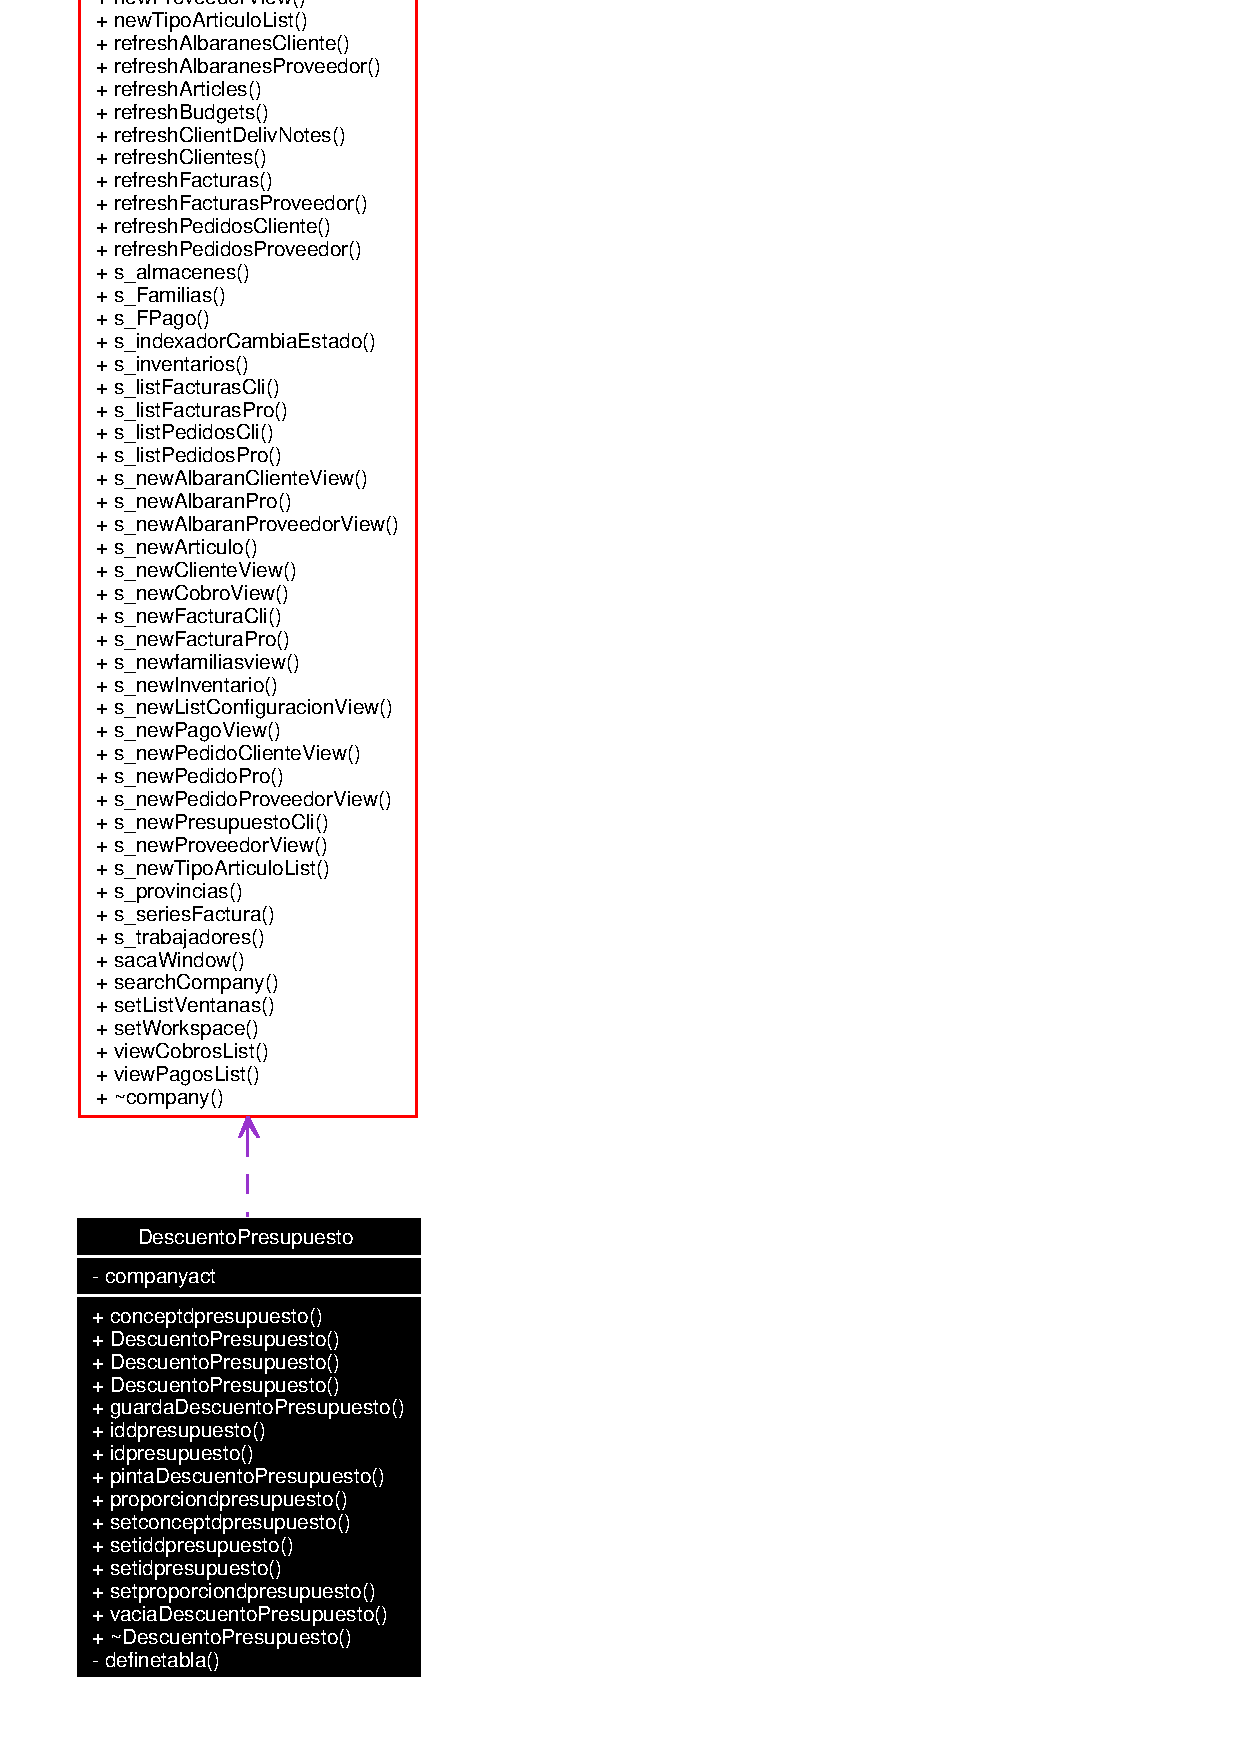
\includegraphics[width=101pt]{classDescuentoPresupuesto__coll__graph}
\end{center}
\end{figure}
\subsection*{M\'{e}todos p\'{u}blicos}
\begin{CompactItemize}
\item 
QString {\bf conceptdpresupuesto} ()\label{classDescuentoPresupuesto_a0}

\item 
{\bf Descuento\-Presupuesto} ({\bf company} $\ast$, QString, QString, QString, QString)
\item 
{\bf Descuento\-Presupuesto} ({\bf company} $\ast$, QString)\label{classDescuentoPresupuesto_a2}

\item 
{\bf Descuento\-Presupuesto} ({\bf company} $\ast$)\label{classDescuentoPresupuesto_a3}

\item 
void {\bf guarda\-Descuento\-Presupuesto} ()\label{classDescuentoPresupuesto_a4}

\item 
QString {\bf iddpresupuesto} ()\label{classDescuentoPresupuesto_a5}

\item 
QString {\bf idpresupuesto} ()\label{classDescuentoPresupuesto_a6}

\item 
virtual void {\bf pinta\-Descuento\-Presupuesto} ()\label{classDescuentoPresupuesto_a7}

\item 
QString {\bf proporciondpresupuesto} ()\label{classDescuentoPresupuesto_a8}

\item 
void {\bf setconceptdpresupuesto} (QString val)\label{classDescuentoPresupuesto_a9}

\item 
void {\bf setiddpresupuesto} (QString val)\label{classDescuentoPresupuesto_a10}

\item 
void {\bf setidpresupuesto} (QString val)\label{classDescuentoPresupuesto_a11}

\item 
void {\bf setproporciondpresupuesto} (QString val)\label{classDescuentoPresupuesto_a12}

\item 
void {\bf vacia\-Descuento\-Presupuesto} ()\label{classDescuentoPresupuesto_a13}

\end{CompactItemize}


\subsection{Descripci\'{o}n detallada}
Administra el descuento en un presupuesto. 



\subsection{Documentaci\'{o}n del constructor y destructor}
\index{DescuentoPresupuesto@{Descuento\-Presupuesto}!DescuentoPresupuesto@{DescuentoPresupuesto}}
\index{DescuentoPresupuesto@{DescuentoPresupuesto}!DescuentoPresupuesto@{Descuento\-Presupuesto}}
\subsubsection{\setlength{\rightskip}{0pt plus 5cm}Descuento\-Presupuesto::Descuento\-Presupuesto ({\bf company} $\ast$, QString, QString, QString, QString)}\label{classDescuentoPresupuesto_a1}


La carga r\'{a}pida tiene un comportamiento poco restrictivo para aumentar la eficiencia. 

La documentaci\'{o}n para esta clase fu\'{e} generada a partir de los siguientes archivos:\begin{CompactItemize}
\item 
descpresupuesto.h\item 
descpresupuesto.cpp\end{CompactItemize}
